%======================================================%
%     ________                            _________    %
%    /  _____/______  ____  __ ________   \______  \   %
%   /   \  __\_  __ \/  _ \|  |  \____ \      /    /   %
%   \    \_\  \  | \(  <_> )  |  /  |_> >    /    /    %
%    \______  /__|   \____/|____/|   __/    /____/     %
%           \/                   |__|                  %
%======================================================%
\documentclass[12pt,a4paper]{report}
\usepackage[left=2cm,right=2cm,top=2cm,bottom=2cm]{geometry}
\usepackage[unicode]{hyperref}
\usepackage[utf8]{vietnam}
\usepackage{amsmath}
\usepackage{amsfonts}
\usepackage{amssymb}
\usepackage{booktabs}
\usepackage{fancyhdr}
\usepackage{fancybox}
\usepackage{graphicx}
\usepackage{hyperref}
\usepackage{indentfirst}
\usepackage{longtable}
\usepackage{lscape}
\usepackage{multirow}
\usepackage{comment} 
\graphicspath{ {./resources/} }
%=======================================================
%\setlength{\parindent}{1cm}
\renewcommand{\baselinestretch}{1.5}


%=======================================================
\newcommand{\Khung}[2]{
    \begin{tabular}{|l|}
        \hline\rule[-2ex]{0pt}{5.5ex}
        \parbox{#1}{#2}\\
        \hline
    \end{tabular}
}
%=======================================================



\begin{document}
    \Khung{0.92\textwidth}{
        \begin{center}
            \normalsize
            \textbf{TRƯỜNG ĐẠI HỌC BÁCH KHOA HÀ NỘI}\\
            \normalsize
            \textbf{VIỆN TOÁN ỨNG DỤNG VÀ TIN HỌC}\\
            \textbf{------------------------------------------------------}\\[0.4cm]
            
\includegraphics[scale=.4]{bk.jpg}\\[1.2cm]
            \textbf{{\large BÁO CÁO TỔNG KẾT MÔN HỌC}}\\[0.3cm]
            \textbf{HỌC PHẦN MI2000 - NHẬP MÔN TOÁN TIN}\\[1cm]
            \textbf{{\large}}\\[0.2cm]
            \textbf{{\large}}\\[3cm]
        \end{center}
       
        \begin{center}
            \normalsize
            \textbf{NHÓM 7 - Lớp CTTN Toán tin K64} \\
            Bùi Tiến Thành - MSSV 20190081 \\
            Phạm Nhật Quang - MSSV 20195910 \\
            Đỗ Mạnh Dũng - MSSV 20195860 \\
            Vũ Minh Hiếu - MSSV 20195872 \\
            
        \end{center}
        \vspace{0.0cm}
        \begin{center}
            \textbf{{\large HÀ NỘI - 2020}}\\
        \end{center}
    }
    \newpage
    \setcounter{page}{2}
    

    \addcontentsline{toc}{chapter}{Mục lục}
    \tableofcontents
    \pagebreak
    
    
    
    %===================================================================================
    \chapter{Tầm quan trong và ứng dụng của Toán Tin}
    \section{Tầm quan trọng của Toán Tin}
    Toán tin (tiếng Anh là Mathematics - Informatics), là ngành học mang tính ứng dụng cao, đặc biệt trong thời đại Công nghệ số như hiện nay \\
    Từ cổ chí kim, con người đã bắt đầu sử dụng toán học. Trải qua nhiều thiên niên kỉ, toán ngày càng trở nên quan trọng trong cuộc sống.  [1]\\
    Một đặc trưng nổi bật trong thời đại chúng ta là sự ứng dụng rộng rãi các phương pháp toán học và khoa học máy tính trong mọi lĩnh vực khác nhau của đời sống,  kinh tế, tài chính, văn hóa, khoa học kỹ thuật, y tế, bảo mật, quản lý, ra quyết định và thiết lập các hệ thống phức tạp v.v.. Chẳng hạn, việc sinh mã có độ tin cậy cao trong truyền dữ liệu dựa trên số học các số nguyên tố. Các mạng truyền thông hiệu quả được thiết kế dựa vào việc sử dụng lý thuyết biểu diễn vô hạn chiều của nhóm. Mạng điện thoại được vận hành thông suốt là do đóng góp không nhỏ của thuật toán đơn hình giải các bài toán qui hoạch tuyến tính. Hệ thống giao dịch tiền điện tử, trong đó có hệ thống ATM mà chúng ta đang sử dụng hàng ngày sẽ không vận hành được nếu thiếu các công cụ đảm bảo an toàn thông tin mà cốt lõi là các thuật toán mã hóa. Các máy chụp cắt lớp hiện đại trong ngành y sẽ không ra đời nếu không có phép biến đổi ngẫu nhiên cùng với các phương pháp giải phương trình với số biến khổng lồ v.v..\newpage
    Cùng với sự phát triển của kinh tế xã hội và khoa học công nghệ, vai trò của toán học và khoa học máy tính cũng như nhu cầu nhân lực ngành Toán Tin ngày càng gia tăng. Theo một nghiên cứu xếp hạng 200 công việc ở Mỹ  vào năm 2014 [2] , một  số công việc có thu nhập cao và môi trường làm việc tốt đều liên quan đến Toán Tin. Cụ thể ngành Toán chiếm vị trí số một, Thống kê chiếm vị trí thứ ba, thứ tư là Kiểm toán, Kĩ sư công nghệ phần mềm xếp thứ bảy, Quản trị hệ thống máy tính đứng thứ tám… Hơn nửa thế kỷ qua, nhiều công ty được xây dựng trên cơ sở toán học đã mở rộng và phát triển mạnh mẽ. Để đáp ứng nhu cầu của xã hội, nhiều trường đại học trên thế giới đã mở các khoa toán ứng dụng và khoa học tính toán. Trong buổi nói chuyện với sinh viên Đại học Bách khoa Hà Nội tại Hội trường C2 vào ngày 22/04/2006, Bill Gates, Chủ tịch tập đoàn Microsoft, đã khẳng định:  “Tôi không thể nào nói hết được tầm quan trọng của công cuộc đào tạo toán học đối với không chỉ máy tính mà với mọi lĩnh vực khác (kinh tế học, kỹ sư). Toán là môn khoa học căn bản nhất. Khi còn trẻ, tôi hiểu được về máy tính là nhờ có một khả năng nhất định về toán. Chúng tôi ứng dụng toán vào trong rất nhiều hoạt động lập trình của mình” và “Các bạn hãy đầu tư lớn hơn cho Toán vì nó sẽ có ý nghĩa trong hầu hết các lĩnh vực”. Theo Jame R.Schatz, người đứng đầu nhóm nghiên cứu tại Cơ quan An ninh quốc gia Hoa Kỳ (NSA), “Đây là thời điểm thích hợp nhất để các bạn trở thành nhà toán học”.\\
    Đó là những chia sẻ đơn giản của những người đã thành công, khẳng định cho tầm quan trọng của toán, đặc biệt là toán ứng dụng. \\
    Không tự nhiên mà Trường Đại học Bách Khoa Hà Nội tính điểm thi đầu vào với môn toán nhân đôi, hay khi xét tuyển KSTN thì môn toán cũng được ưu tiên xét trước. Toán là môn khoa học cơ bản, nó được áp dụng vào nhiều ngành học khác. Hầu như toàn bộ các ngành học đền cầu đến nó. Những bài tập Lí, Hóa hay lớn hơn là những công trình đồ sộ, hoặc đưa con người ra ngoài vũ trụ thì đều cần được tính toán kĩ càng.  “Không có lĩnh vực khoa học nào thâm nhập và ảnh hưởng đến các lĩnh vực của cuộc sống và công việc như Toán học. Từ chế tạo ô tô đến phân làn đường, từ mua bán trong siêu thị đến kiến trúc, từ dự báo thời tiết đến nghe MP3, từ đi tàu đến Internet – tất cả đều là Toán học!”\\ Chừng đó là đủ để thấy tầm quan trọng của Toán trong cuộc sống. Tóm lại, bản chất gốc rễ của khoa học kĩ thuật: Chính là Toán!\\ Bên cạnh đó, một trong những ứng dụng lớn nhất của Toán, chính là thứ mà cả thế giới đang đổ dồn sự chú ý về nó: Tin học.\\ Tin học là một ngành khoa học chuyên nghiên cứu quá trình tự động hóa việc tổ chức, lưu trữ và xử lý và truyền dẫn thông tin của một hệ thống máy tính cụ thể hoặc trừu tượng (ảo). Với cách hiểu hiện nay, tin học bao hàm tất cả các nghiên cứu và kỹ thuật có liên quan đến việc mô phỏng, biến đổi và tái tạo thông tin.

    Tin học xem xét sự tương tác giữa con người và thông tin bên cạnh việc xây dựng giao diện, tổ chức, công nghệ và hệ thống. Như vậy, tin học có bề rộng lớn và bao gồm nhiều chuyên ngành, bao gồm các ngành khoa học máy tính, hệ thống thông tin, công nghệ thông tin và thống kê. Kể từ khi máy tính ra đời, các cá nhân và tổ chức ngày càng xử lý thông tin kỹ thuật số. Điều này đã dẫn đến việc nghiên cứu về tin học với các khía cạnh tính toán, toán học, sinh học, nhận thức và xã hội, bao gồm cả nghiên cứu về tác động xã hội của công nghệ thông tin. \\ Tin học có lợi thế về sự nhanh chóng, chính xác, là một người giúp việc đa năng cho con người. Ngày nay mọi vấn đề quan trọng trên thế giới hầu như được giải quyết bằng máy tính - thứ có thể coi là biểu tượng của tin học. Và với mạng lưới người sử dụng phủ sóng toàn cầu, đại đa số cư dân xung quanh thế giới đều đang dùng thì có thể dễ dàng thấy được rằng chúng ta đang sống cùng tin học. Thiết bị tin học đang ngày càng được cải tiến, không còn cồng kềnh, khó sử dụng mà nhỏ gọn, thân thiện với cả những người dùng bình thường nhất.\\ Có người nói rằng:"Tin học thực ra cũng chỉ là Toán học biểu diễn theo một kiểu khác", nó cho thấy mối quan hệ mật thiết giữa toán học và tin học. Và nếu như toán học đã là xương sống của nhân loại từ rất lâu thì tin học cũng đang từng bước biến mình trở thành nhịp thở của cuộc sống này. Tóm lại, ứng dụng tin học trong nhu cầu đời sống là cần thiết và có ý nghĩa thiết thực. Thông qua sự phát triển của tin học hàng loạt các lĩnh vực khác được hỗ trợ hiệu quả, giải quyết được nhiều bài toán hóc búa trong sản xuất, kinh doanh, học tập.\newpage
    \section{Ứng dụng của Toán Tin}
    Quan trọng là thế, nhưng để mang được ứng dụng của Toán vào đời sống thì không hề dễ dàng. Có một thời người ta tưởng rằng làm Toán ứng dụng dễ hơn làm Toán lý thuyết, vì làm lý  thuyết phải nghĩ ra cái mới còn làm ứng dụng chỉ cần biết “tiêu hóa” những điều  đã biết. Trên thực tế, những người đã có ít nhiều kinh nghiệm đều biết rằng đây là lĩnh vực “nói thì dễ mà làm thì khó”. Ở nước ta thì phần “nói” thì đã được triển khai từ lâu rồi, còn phần “làm” thì hầu như “còn nguyên”! Vì sao?\\
    \textbf{Toán ngày nay không “đi trực tiếp”  được vào thực tiễn}\\
    Đã qua rồi thời kỳ của những ứng dụng toán học tuần túy, theo kiểu chỉ cần biết đến toán là xong… Toán học ngày nay không mấy khi “đi thẳng” được vào thực tiễn, mà thường phải “ăn theo” một số công nghệ khác, cho nên người làm ứng dụng toán phải có khả năng tiếp cận các công nghệ mới (công nghệ phần mềm, công nghệ tính toán hiệu năng cao, điện tử, tự động hóa, số hóa,…). Thêm nữa, muốn ứng dụng toán học vào lĩnh vực nào thì phải có hiểu biết đủ tốt về lĩnh vực đó (xử lý hình ảnh, âm thanh, môi trường, sinh thái…) và cũng có nghĩa là phải học thêm một ngành mới ngoài toán. Đây chính là những điều mà phần lớn những người làm toán ngại nhất.\\
    \textbf{Từ  “Toán lý thuyết” đến “Toán ứng dụng được” là một quãng đường dài}\\
    Phần lớn những người làm toán lý thuyết chưa nhìn thấy những khó khăn đặc thù của công tác ứng dụng. Ví dụ, không ít người tưởng rằng đó chỉ đơn thuần là việc áp dụng những kết quả có sẵn trong lý thuyết vào việc giải quyết một vấn đề gì đó đặt ra trong thực tiễn, mà không biết rằng cái kết quả lý thuyết ấy chỉ là cái “phần nổi của tảng băng chìm”. Hãy lấy hệ mật mã RSA làm ví dụ. Không ít người cho rằng chỉ cần biết về tính “bất khả ngược” của phép nhân hai số nguyên tố lớn là đủ để thiết lập được hệ mã RSA. Tuy nhiên, nếu là người “trong nghề” làm mật mã thì biết rằng có bao nhiêu cạm bẫy giăng ra xung quanh hệ mã đó và chỉ cần một chút sơ suất nhỏ là đủ dẫn đến thiệt hại vô cùng lớn (Điều này đã được nhiều nhà mật mã trên thế giới nói đến). Đây là nguyên nhân khiến cho việc mã hóa theo sơ đồ lý thuyết chỉ mang tính hình thức, còn để triển khai vào thực tiễn người ta phải dày công nghiên cứu ra những lược đồ khác hẳn. Ta hiểu vì sao chính những nhà toán học được xem là “chuyên gia lão luyện” về Toán trong mật mã (như Koblitz, Menezes…) đã dùng thuật ngữ “lược đồ sách vở” (text book scheme) để chỉ những lược đồ mã hóa trong sách giáo khoa. Như vậy, ở đây ta cũng gặp tình huống giống như trong nhiều lĩnh vực khác, như Giải tích Fourier hay Đại số tuyến tính: Cơ sở lý thuyết của Giải tích Fourier có thể được trình bày trong khuôn khổ một chương của giáo trình Giải tích Toán học, nhưng để ứng dụng được thì người ta cần tới phép Biến đổi Fourier nhanh mà việc trình bày có thể cần cả một cuốn sách dày hơn cả giáo trình Giải tích Toán học. Tương tự như vậy, giáo trình Đại số tuyến tính (bậc đại học) có thể dễ dàng “nuốt trôi” trong một học kỳ, nhưng khi vào thực tế thì sẽ thấy rằng chỉ riêng một góc “phương trình tuyến tính cỡ lớn” cũng đủ để mà “vật lộn” cả năm trời không hết. Tóm lại, từ cái Toán “lý thuyết” trong sách giáo khoa đến cái Toán “dùng được” trong thực tiễn là còn cả một con đường dài.\\
    \textbf{Toán ứng dụng mang tính “liên ngành”}\\
    Để làm lý thuyết, thông thường người ta chỉ cần biết về chuyên ngành hẹp mà mình nghiên cứu, còn để làm ứng dụng thì phải có tầm hiểu biết đủ sâu về chuyên ngành rộng. Điều này cũng được thể hiện rất rõ trong lĩnh vực mật mã. Ít khi người làm về lý thuyết số và hình học đại số  phải đọc để biết về hàm Bull, về xác suất thống kê… Nhưng muốn ứng dụng được các thành tựu của lý thuyết số và hình học đại số vào lý thuyết mật mã phi đối xứng thì không thể không biết các lĩnh vực này. Có thể nói rằng, cái khó trong việc nắm bắt cho đủ kiến thực để làm ứng dụng không hề thua kém cái khó trong việc tìm ra cái mới (có ý nghĩa thực sự) đối với người làm lý thuyết.\\
     Khó khăn là thế, nhưng tách rời Toán và ứng dụng của nó là điều không tưởng. Toán học như một chú bạch tuộc khổng lồ, mà xúc tu của nó chạm tới mọi góc cạnh của cuộc sống.
     
    \begin{itemize}
        \item Đầu tiên phải nhắc tới những ngành khoa học kĩ thuật: Điện tử Viễn thông, Tự động hóa, Khoa học /kĩ thuật máy tính, Cơ Điện tử,... đều áp dụng toán để tạo ra những sản phẩm có tính thực tiễn rất cao như điện thoại, máy tính, dây chuyền sản xuất, robot, trò chơi điện tử, mạng xã hội, hệ thống bảo mật...
        \item Tiếp theo đó là trong kinh tế. Toán kinh tế là môn khoa học nhằm vận dụng toán học trong phân tích các mô hình kinh tế để từ đó hiểu rõ hơn các nguyên tắc và các quy luật kinh tế của nền kinh tế thị trường. Toán kinh tế cung cấp cho các Nhà Quản lý các kiến thức để họ có thể vận dụng vào việc ra các quyết định sản xuất. Toán kinh tế còn được hiểu là phương pháp tiếp cận dưới hình thức toán học của khoa học kinh tế. Nó giúp kinh tế học diễn giải, trình bày được nhiều vấn đề mà phương pháp diễn giải bằng lời thông thường không có hiệu quả. 
        \item Trong giáo dục, ngoài việc dạy và học môn Toán, Toán còn giúp giải quyết nhiều bài Vật lí, Hóa học hay Sinh học...
        \item Trong Địa lí thực tế, Toán học giúp đo độ cao ngọn núi hay tính tuổi của mẫu vật. Đó mới chỉ là một phần rất nhỏ trong ứng dụng của Toán học trong thực tiễn. 
    \end{itemize}
     
    {\textbf{*Với những ứng dụng cụ thể của Toán Tin trong Tin học có thể kể đến:}} \\
    
     1..\textbf{Thông qua sự phát triển của tin học, lĩnh vực giải trí trở nên tiện ích hơn} \\Mỗi ngày chúng ta xem video, chơi điện tử hay sử dụng các ứng dụng trên di động, laptop… đó là nhờ những tác dụng hữu ích của tin học mang lại. Nhờ có các phần mềm thông minh, chúng ta xem phim, nghe nhạc, xem các chương trình giải trí góp phần giảm bớt căng thẳng trong cuộc sống.\\Ngoài ra, chuyên gia công nghệ còn sáng tạo ra các mạng xã hội như Facebook, Instagram,… cho phép người dùng trao đổi thông tin, tán ngẫu, truyền tải thông tin, hình ảnh,…Có thể nói lĩnh vực giải trí trở nên khởi sắc và hữu ích hơn nhờ có sự hỗ trợ của công nghệ thông tin hỗ trợ. Ứng dụng tin học tham gia vào hỗ trợ lao động trí óc vừa giúp con người giải trí, thư giãn cuộc sống.\\
     \textbf{Vai trò ứng dụng tin học trong học tập, mở mang tri thức}\\
     Khoa học IT phát triển và chiếm vị thế nòng cốt trong đời sống, ngành giáo dục cũng được hưởng lợi từ lĩnh vực này. Nhờ sự phát triển lĩnh vực tin học hoạt động giảng dạy trở nên hiệu quả hơn. Thông qua các bài giảng sinh động bằng hình ảnh, video khiến học sinh cảm thấy lĩnh hội kiến thức nhanh, kích thích não bộ suy nghĩ, ham học hỏi.\\Đối với học sinh, thay vì trực tiếp đến nhờ thầy cô giảng bài có thể truy cập internet xem các bài giảng sẵn có trên ứng dụng Youtube. Qua đó sinh viên, học sinh tự tìm hiểu tri thức thông qua mạng, phân tích vấn đề về buổi học hôm trước cũng như sẵn sàng tiếp thu kiến thức cho ngày hôm sau. Đồng thời tin học ứng dụng còn tạo ra động lực giúp học sinh sáng tạo tìm kiếm ra luồn tri thức mới. Đối với cấp bậc Cao đẳng/ Đại học, tin học mang lại khả năng học tập, nghiên cứu và mở ra cơ hội phát triển bản thân.\\
     \textbf{Ứng dụng tin học trong học tập, nghiên cứu ngành y}\\
     Nhờ trình độ phát triển tin học,lĩnh vực y học đạt được bước tiến lớn trong cứu chữa và điều trị bệnh cho con người. Quy trình khám, chuẩn đoán bệnh diễn ra nhanh chóng, hiệu quả. Quy trình gồm: các công cụ tin học sẽ kiểm tra, soi xét, chụp chiếu, cung cấp các thông số để bác sĩ biết được và đưa ra kết luận về tình trạng sức khỏe cho bệnh nhân.\\Đối với hoạt động điều trị bệnh hay phẫu thuật đang chứng minh ứng dụng tin học trong đời sống mang lại hiệu quả thiết thực. Các hoạt động mà tin học thâm nhập phải kể đến như mổ và cấy ghép các bộ phận cơ thể người, cắt khối u,… nghiên cứu phát triển thuốc. Ngoài ra nhờ ứng dụng tin học góp phần giảm tải các thủ tục hành chính cồng kềnh, giúp cho việc quản lý hồ sơ bệnh nhân gọn tiện hơn,…\\
     \newline
     \newline
     \textbf{Dựa vào sự phát triển của tin học mở ra cơ hội tìm kiếm việc làm và tuyển dụng nhân tài}\\
     Nếu bạn đang có nhu cầu tìm kiếm việc làm chỉ cần lên Google gõ: bí kíp tìm việc làm, tìm việc làm nhanh,… sẽ ra rất nhiều kết quả. Ngoài ra, biết cách sử dụng thuần thục các ứng dụng tin học về mạng xã hội hay các wesbite tuyển dụng, cơ hội “săn” được việc làm như ý khá cao. Việc ứng dụng tin học vào rong tìm kiếm công việc giúp chúng ta tiết kiệm thời gian và công sức hơn, đồng thời những trao đổi tương tác với nhà tuyển dụng sẽ thuận tiện hơn.\\Đối với các công ty, tổ chức kinh doanh,… nếu có nhu cầu tuyển dụng lao động có thể đăng lên các wesbite hoặc mạng xã hội tìm kiếm ứng viên. Một lưu ý rằng cần nêu ra những yêu cầu cụ thể đối với người ứng tuyển, nhà tuyển dụng đã có thể khoanh vùng được ứng nhân tài. Hiện nay, hoạt động tuyển dụng thông qua ứng dụng tin học đang cho thấy độ phổ biến và hiệu quả cao.\\
     \textbf{Ứng dụng tin học trong học tập việc quản lý, công tác hành chính}\\
     Thật đơn giản cho những người làm CEO, hoặc là nhà quản lý muốn gám sát nhân viên, theo dõi công việc và ngân sách…. Chỉ cần tải hoặc mua phần mềm giám sát, quản lý từ các nhà sản xuất là bạn có thể biết đươc hàng trăm nghìn người lao động trong tổ chức kinh doanh. Trong vài năm trở lại đây các công ty có xu hướng tung ra thị trường các phần mềm quản lý với những tính năng và giá cả khác biệt, đặc thù hóa cho từng ngách nhỏ. Một số phần mềm miễn phí trong công tác quản lý như: Google Sheet, Trello, Toko…\\ Nhờ tin học phát triển nên các lĩnh vực thương mại điện tử ngày càng có xu hướng gia tăng. Đây có thể coi ứng dụng tin học trong đời sống một cách mạnh mẽ và rõ rệt nhất. Hoạt động mua bán, trao đổi, mời chào, các dịch vụ quảng cáo, content mở rộng như vũ bão.\\
     \textbf{Sự phát triển của tin học góp phần hỗ trợ hoạt động quốc phòng – an ninh}\\
     Vào những thế kỷ trước phương thức truyền thư tay thông qua bưu điện rất thịnh hành, ngày này internet đã thay thế tất cả. Facebook hay Messenger giúp các cán bộ chiến sĩ truyền tải thông điệp, giao lưu tin tức với nhau nhanh chóng. Chẳng hạn ứng dụng đám mây Skype hỗ trợ những người lính có thể gửi thông tin trực tiếp với nhau, gửi các bí mật thông tin một cách an toàn, nhanh chóng. Ngoài ra công tác quản lý số liệu, thống kê lực lượng diễn ra hiệu quả hơn nhờ có các công cụ tin học hỗ trợ.\\Nhờ có tin học cũng như công nghệ, những chiến sĩ hoạt động trong công tác bảo vệ đất nước sẽ nắm bắt thông tin nhanh chóng, kịp thời. Kể cá những nguồn tin chính trị khẩn cũng cập nhật nhanh. Qua đó các phương thức truyền tin thủ công sẽ được thay thế bằng phương thức hiện đại thông qua kết nối internet.\\
     \textbf{Lĩnh vực ngân hàng cũng được lợi nhờ sự phát triển của tin học}\\
     Ngoài các lĩnh vực kể trên, ứng dụng tin học vào hoạt động tài chính cho thấy nhiều dấu hiệu tốt đẹp. Điển hình như trong tổ chức tài chính, để biết được về hoạt động của khách hàng, người lao động ngân hàng phải tìm thông tin cá nhân của khách hàng như họ tên, số di động, hoặc sốtiền trong thẻ có thể biết được đích danh vị khách hàng, đã thực hiện lúc nào và lấy bao nhiêu trong tài khoản.\\  
     Liên quan đến ngành kiểm toán thời gian trước nhiều nhân viên kế toán luôn căng thẳng bởi các thông số nhưng thông qua ứng dụng tin học, các thao tác trở nên nhanh và hiệu quả hơn. Giờ đây ngân hàng nào biết ứng dụng tin học thực hiện thao tác thủ tục giấy tờ nhanh gọn cũng như bảo mật an toàn sẽ chiếm ưu thế.\\





    
    
    
    %===================================================================================
    \chapter{Cơ hội việc làm và du học}
    \section{Cơ hội việc làm}
    \begin{figure}[h]
    	\centering
    		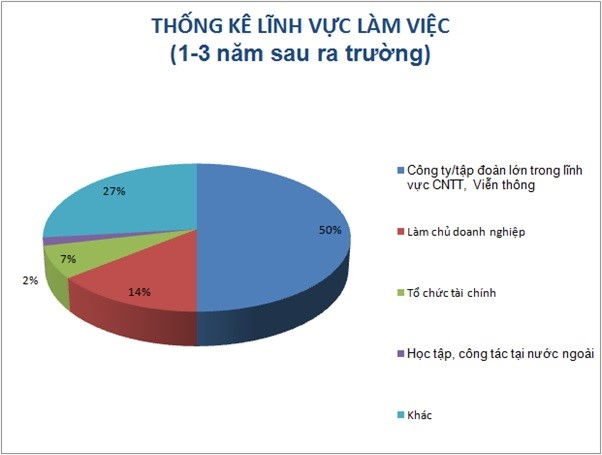
\includegraphics[scale=1]{1.jpg}
    			\caption{Thống kê việc làm sau ra trường ngành Toán Tin năm 2014}
    \end{figure}

    \newpage
        Sau khi tốt nghiệp, sinh viên có thể công tác trong nhiều ngành nghề có sử dụng kiến thức Toán học ứng dụng và Tin học, như:
      \begin{itemize}
       \item{\bf1. Chuyên viên phân tích đầu tư}
        
    Việc theo dõi những thăng trầm của thị trường tài chính có tạo cho bạn cảm giác hồi hộp không? Các nhà phân tích đầu tư sẽ nghiên cứu xu hướng kinh tế và đánh giá các cơ hội đầu tư cho các ngân hàng, tổ chức chứng khoán và các công ty bảo hiểm. Để thành công trong lĩnh vực này, bạn phải có kiến thức toán học, khả năng đánh giá mức độ rủi ro và tính toán giá trị của các khoản đầu tư khác nhau cũng như kỹ năng phân tích các kết quả đã nghiên cứu. Các công ty tài chính, bảo hiểm, chứng khoán hay ngân hàng là nơi làm việc lý tưởng cho vị trí này.
    
    \item{\bf{2.Chuyên viên kế hoạch tài chính }}
    
    Chuyên viên kế hoạch tài chính có thể làm việc cho công ty, đoàn thể hoặc cho cá nhân. Tại công ty, chuyên viên kế hoạch tài chính sẽ phụ trách lập kế hoạch và đánh giá thu-chi tài chính định kỳ theo yêu cầu của cơ quan, đơn vị; đánh giá nhanh các số liệu và kiểm soát chất lượng giải ngân theo định kỳ. Khi làm việc với các cá nhân, chuyên viên kế hoạch tài chính có thể giúp cấu trúc các khoản đầu tư của các cá nhân cho từng mục tiêu cụ thể. Theo đó, họ cần có kỹ năng giao tiếp, khả năng thiết lập niềm tin với khách hàng cùng với một nền tảng toán học vững chắc. Chuyên viên kế hoạch tài chính có thể làm việc tại các ngân hàng, các công ty cung cấp dịch vụ tài chính, các dự án, … 
    \item{\bf 3. Chuyên viên phân tích nghiên cứu hoạt động}
    
    Kỹ năng phân tích đóng vai trò rất quan trọng đối với công việc của các nhà phân tích nghiên cứu hoạt động. Họ áp dụng phân tích thống kê cho các chức năng nghiệp vụ và sử dụng các kỹ thuật mô hình toán học để tìm ra cách một tổ chức có thể hoạt động hiệu quả hơn. Chẳng hạn, một chuyên viên phân tích nghiên cứu hoạt động có thể giúp các hãng hàng không phát triển lịch bay hoặc giúp các nhà sản xuất máy tính tối ưu hóa quy trình sản xuất của họ. Các đơn vị làm việc cho vị trí chuyên viên phân tích nghiên cứu hoạt động tương đối rộng khắp, từ các cơ quan chính phủ, tổ chức phi chính phủ, cho tới các công ty tư nhân nội địa và quốc tế. 
    \item{\bf4. Kỹ sư hệ thống}
    
    Các cử nhân Toán Ứng dụng, đặc biệt là chuyên ngành Toán – Tin, sau khi ra trường có thể đảm nhiện vị trí kỹ sự hệ thống tại các công ty điện tử và truyền thông, mà chìa khóa cho công việc này chính là kỹ năng phân tích dữ liệu và giải quyết vấn đề. Khi làm việc tại các cơ quan này, bạn cũng có nhiều cơ hội để tiếp cận và học hỏi các công nghệ điện tử mới nhất, qua đó bắt kịp với xu thế phát triển công nghệ của đất nước và thế giới. Các đơn vị làm việc tiêu biểu cho vị trí này như các công ty IT như TOPICA, Framgia, hay các công ty viên thông như Viettel, VNPT,...
    \item{\bf5. Chuyên viên phân tích ngân sách}
    
    Khi các cơ quan chính phủ, các công ty nghiên cứu hoặc các tổ chức học thuật cần phải quyết định cách phân bổ kinh phí giữa các dự án khác nhau, họ thường tìm tới các nhà phân tích ngân sách. Các chuyên gia này phân tích các chi phí gắn liền với các đề xuất ngân sách khác nhau và xác định tác động tiềm năng của chúng đối với tình trạng tài chính tổng thể của một tổ chức. Sau đó, họ đưa ra các khuyến nghị tài trợ dựa trên những phát hiện của họ. Làm việc tại vị trí này, ứng viên cần có kiến thức vững chắc về toán học, tài chính và kỹ năng phân tích. Hầu hết các nhà tuyển dụng tìm kiếm các ứng cử viên với bằng cử nhân ngành Toán Ứng dụng, nhưng một số yêu cầu bằng Thạc sĩ.
    \item{\bf6. Kế toán}
    
    Cân bằng sổ sách của tổ chức và cập nhật hồ sơ tài chính là trách nhiệm của kế toán. Người làm việc tại vị trí này phụ trách tính toán biên chế, chuẩn bị tờ khai thuế và đảm bảo rằng công ty tuân thủ tất cả các quy tắc và quy định tài chính. Đây là vị trí tối quan trọng trong tất cả các cơ quan, công ty. Với kiến thức về Toán học và thống kê, cộng với sự tỉ mỉ, cẩn thận, cử nhân ngành Toán Ứng dụng hoàn toàn có thể đảm nhiệm vị trí kế toán tại các cơ quan, đơn vị. 
    \item{\bf7. Lập trình viên}
    
    Tâm bằng cử nhân về toán học, đặc biệt là chuyên ngành Toán – Tin có thể giúp bạn có được vị trí của một lập trình viên tại một số công ty công nghệ. Vị trí này có thể liên quan đến việc viết các đặc tả cho các ứng dụng phần mềm, thiết kế các truy vấn cơ sở dữ liệu, hoặc phát triển các thủ tục kiểm thử và gỡ lỗi. Bạn cũng có thể đảm nhiệm tùy chỉnh một phần mềm để đáp ứng các nhu cầu cụ thể của công ty hoặc khách hàng của bạn. Các kiến thức về toán tin, các ngôn ngữ lập trình và hệ điều hành sẽ giúp bạn phát triển trong lĩnh vực này. 
    \item{\bf8. Chuyên viên thống kê}
    
    Nói chung, các chuyên viên thống kê thu thập và phân tích dữ liệu để xác định hướng giải quyết vấn đề. Vị trí này sẽ tiến hành các hình thức thu thập dữ liệu như khảo sát qua điện thoại, bảng câu hỏi trực tuyến hoặc thử nghiệm, từ đó phân tích và rút ra kết luận dựa trên kết quả. Theo đó, chuyên viên thống kê cần có kiến thức về toán học, thống kê, kế toán hay quản trị kinh doanh. Chuyên viên thống kê có thể làm việc cho các cơ quan chính phủ, viện nghiên cứu, công ty bảo hiểm, công ty dược phẩm hoặc thậm chí là các tổ chức thể thao. 
    \item{\bf9. Nhà toán học}
    
    Một nhà toán học là một người thích giải quyết vấn đề thông qua phân tích các con số như nghiên cứu các lý thuyết và khái niệm mới hay phát triển các mô hình toán học. Nhà toán học tham gia giải quyết những vấn đề toán học nằm ngoài phạm vi toán học thuần túy thì được gọi là nhà toán học ứng dụng. Những người này dùng kiến thức chuyên môn và phương pháp luận chuyên ngành để tiếp cận nhiều vấn đề nổi bật hiện diện trong các ngành khoa học có liên quan như khoa học, kỹ thuật, kinh doanh. Các đơn vị nghiên cứu học thuật như Viện Toán học thuộc Viên Hàn Lâm Khoa học Công nghệ Việt Nam là địa điểm làm việc lý tưởng. 
    
    \item{\bf10. Giảng viên/Giáo viên toán học} 
    
    Đây là công việc phù hợp cho các ứng viên yêu thích thử thách toán học đối với sinh viên, học sinh ở các độ tuổi và khả năng khác nhau. Bạn có thể giúp các học viên trẻ nắm vững các khái niệm liên quan đến đại số, hình học và phép tính. Bằng cử nhân ngành Toán Ứng dụng là “tấm vé” giúp bạn thực hiện ước mơ sư phạm và toán học của mình.
    
    
    \end{itemize}
    Cùng với sự phát triển của kinh tế xã hội và khoa học công nghệ, vai trò của toán học và khoa học máy tính cũng như nhu cầu nhân lực ngành Toán Tin ngày càng gia tăng.  Theo một nghiên cứu xếp hạng 200 công việc ở Mỹ  vào năm 2014, một  số công việc có thu nhập cao và môi trường làm việc tốt đều liên quan đến Toán Tin. Cụ thể, ngành Toán đứng vị trí số một, Thống kê  đứng vị trí thứ ba, thứ tư là Kiểm toán, Kĩ sư công nghệ phần mềm xếp thứ bảy, Quản trị hệ thống máy tính đứng thứ tám.  Theo Jame R.Schatz, người đứng đầu nhóm nghiên cứu tại Cơ quan An ninh quốc gia Hoa Kỳ (NSA), “Đây là thời điểm thích hợp nhất để các bạn trở thành nhà toán học”.
    \newpage
    \section{Cơ hội du học}
    \begin{figure}[h]
        	\centering
        		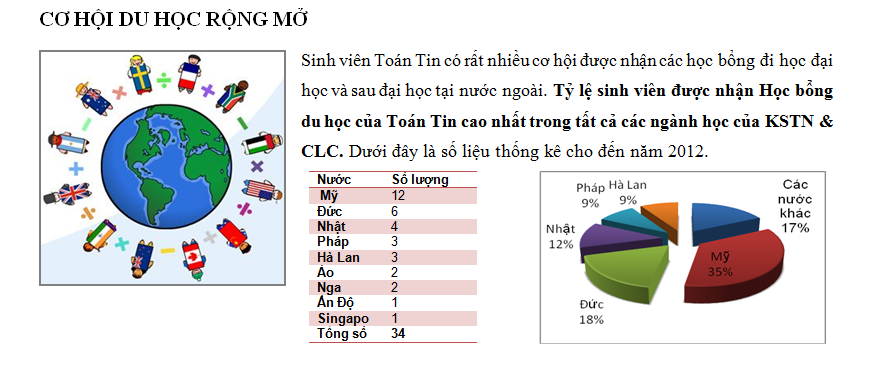
\includegraphics[scale=0.75]{2.png}
        			\caption{Cơ hội du học ngành Toán Tin}
    \end{figure}
    
    Sinh viên Toán Tin có rất nhiều cơ hội nhận học bổng đại học, sau đại học ở nước ngoài, đặc biệt là học bổng sau đại học.Riêng ở Hoa Kỳ, đã có \textbf{khoảng 12.000 suất} học bổng. Ngoài Hoa Kỳ, sinh viên Toán Tin còn có thể theo học ở các quốc gia khác, điển hình như:
    
    \begin{itemize}
        \item Nhật Bản
        \item Hàn Quốc
        \item Singapore
        \item Đức
        \item Pháp
    \end{itemize}
    
    
    %===================================================================================
    \chapter{Chương trình đào tạo của hệ Tài năng Toán - Tin}
    \section{Giới thiệu chung}
    
    Chương trình đào tạo của hệ Tài năng Toán - Tin đào tạo mô hình tích hợp Cử nhân + Thạc sĩ (4 + 1.5 năm) của trường ĐHBK Hà Nội, có nhiều lựa chọn về ngành học và hướng phát triển nghề nghiệp theo nguyện vọng và năng lực cá nhân. Chương trình gồm 8 khối:
    
    \begin{itemize}
        \item Khối kiến thức Lý luận chính trị + Pháp luật đại cương (13TC)
        \item Khối kiến thức Giáo dục thể chất (5TC)
        \item Khối kiến thức Giáo dục Quốc phòng - An ninh (165 tiết)
        \item Khối kiến thức Khối kiến thức Toán và Khoa học cơ bản (33TC)
        \item Khối kiến thức Cơ sở và cốt lõi ngành (47TC)
        \item Khối kiến thức Kiến thức bổ trợ xã hội (9 TC)
        \item Khối kiến thức Tự chọn theo định hướng (16TC) với 4 module:
            \begin{itemize}
                \item Module 1: Tính toán và hệ thống phần mềm
                \item Module 2: Xử lý dữ liệu thông minh
                \item Module 3: Tính toán khoa học
                \item Module 4: Toán ứng dụng trong kinh tế và công nghiệp
            \end{itemize}
        \item Thực tập kỹ thuật và Đồ án tốt nghiệp Cử nhân (8TC)
    \end{itemize}
    
%=============================================BEGIN TABLE=============================================
    % Please add the following required packages to your document preamble:
    % \usepackage{multirow}
    % \usepackage{lscape}
    % \usepackage{longtable}
    % Note: It may be necessary to compile the document several times to get a multi-page table to line up properly

    \begin{landscape}
    
        \section{Các khối kiến thức}
    
        \textit{(So với chương trình chuẩn, bảng tổng hợp chương trình đào tạo đã có một số thay đổi nhỏ trong khối kiến thức GDTC và Lý luận chính trị, với các học phần đã thay đổi theo chương trình được niêm yết trên SIS của chúng em)}
    
        \begin{longtable}[c]{|c|c|c|c|c|c|c|c|c|c|c|c|}
        \hline
        \multicolumn{12}{|c|}{\textbf{CỬ NHÂN HỆ THỐNG TOÁN TIN}}                                                                                                                                                                                                                                                                             \\ \hline
        \endhead
        %
        \multirow{2}{*}{\textbf{STT}} & \multirow{2}{*}{\textbf{Mã số}} & \multirow{2}{*}{\textbf{Tên HP}}                             & \multirow{2}{*}{\textbf{\begin{tabular}[c]{@{}c@{}}KHỐI LƯỢNG\\  (TC)\end{tabular}}} & \multicolumn{8}{c|}{\textbf{KỲ HỌC THEO KHHT CHUẨN}}                                                          \\ \cline{5-12} 
                                      &                                 &                                                              &                                                                                      & \textbf{1}  & \textbf{2}  & \textbf{3}  & \textbf{4}  & \textbf{5}  & \textbf{6}  & \textbf{7}  & \textbf{8}  \\ \hline
        \multicolumn{3}{|c|}{\textbf{Lý luận chính trị + Pháp luật đại cương}}                                                         & \textbf{13}                                                                          &             &             &             &             &             &             &             &             \\ \hline
        1                             & SSH1111                         & Triết học Mác - Lênin                                        & 3                                                                                    &             & 3           &             &             &             &             &             &             \\ \hline
        2                             & SSH1121                         & Kinh tế chính trị Mác - Lênin                                & 2                                                                                    &             &             & 2           &             &             &             &             &             \\ \hline
        3                             & SSH1131                         & Chủ nghĩa xã hội khoa học                                    & 2                                                                                    &             &             &             & 2           &             &             &             &             \\ \hline
        4                             & SSH1141                         & Lịch sử Đảng cộng sản Việt Nam                               & 2                                                                                    &             &             &             &             & 2           &             &             &             \\ \hline
        5                             & SSH1151                         & Tư tưởng Hồ Chí Minh                                         & 2                                                                                    &             &             &             &             & 2           &             &             &             \\ \hline
        6                             & EM1170                          & Pháp luật đại cương                                          & 2                                                                                    & 2           &             &             &             &             &             &             &             \\ \hline
        \multicolumn{3}{|c|}{\textbf{Giáo dục thể chất (5TC)}}                                                                         &                                                                                      &             &             &             &             &             &             &             &             \\ \hline
        1                             & PE1014                          & Lý luận TDTT                                                 & (0-0-2-0)                                                                            & x           &             &             &             &             &             &             &             \\ \hline
        2                             & PE1024                          & Bơi lội                                                      & (0-0-2-0)                                                                            & x           &             &             &             &             &             &             &             \\ \hline
        3                             & PE1010                          & Giáo dục thể chất A                                          & (0-0-2-0)                                                                            &             & x           &             &             &             &             &             &             \\ \hline
        4                             & PE1020                          & Giáo dục thể chất B                                          & (0-0-2-0)                                                                            &             &             & x           &             &             &             &             &             \\ \hline
        5                             & PE1030                          & Giáo dục thể chất C                                          & (0-0-2-0)                                                                            &             &             &             & x           &             &             &             &             \\ \hline
        \multicolumn{3}{|c|}{\textbf{Giáo dục Quốc phòng - An ninh (165 tiết)}}                                                        &                                                                                      &             &             &             &             &             &             &             &             \\ \hline
        1                             & MIL1110                         & Đường lối quân sự của Đảng                                   & 0(3-0-0-6)                                                                           & x           &             &             &             &             &             &             &             \\ \hline
        2                             & MIL1120                         & Công tác quốc phòng, an ninh                                 & 0(3-0-0-6)                                                                           &             & x           &             &             &             &             &             &             \\ \hline
        3                             & MIL1130                         & QS chung và chiến thuật, kỹ thuật bắn súng tiểu liên AK, CKC & 0(3-2-0-8)                                                                           &             &             & x           &             &             &             &             &             \\ \hline
        \multicolumn{3}{|c|}{\textbf{Khối kiến thức Toán và Khoa học cơ bản}}                                                          & \textbf{33}                                                                          &             &             &             &             &             &             &             &             \\ \hline
        1                             & MI1111                          & Giải tích I                                                  & 4(3-2-0-8)                                                                           & 4           &             &             &             &             &             &             &             \\ \hline
        2                             & MI1121                          & Giải tích II                                                 & 3(2-2-0-6)                                                                           &             & 3           &             &             &             &             &             &             \\ \hline
        3                             & MI1131                          & Giải tích III                                                & 3(2-2-0-6)                                                                           &             & 3           &             &             &             &             &             &             \\ \hline
        4                             & MI1141                          & Đại số                                                       & 4(3-2-0-8)                                                                           & 4           &             &             &             &             &             &             &             \\ \hline
        5                             & MI3030                          & Xác suất thống kê                                            & 4(3-2-0-8)                                                                           &             &             & 4           &             &             &             &             &             \\ \hline
        6                             & PH1110                          & Vật lý đại cương I                                           & 3(2-1-1-6)                                                                           &             & 3           &             &             &             &             &             &             \\ \hline
        7                             & PH1120                          & Vật lý đại cương II                                          & 3(2-1-1-6)                                                                           &             &             & 3           &             &             &             &             &             \\ \hline
        8                             & IT1110                          & Tin học đại cương                                            & 4(3-1-1-8)                                                                           &             &             & 4           &             &             &             &             &             \\ \hline
        9                             & MI3010                          & Toán rời rạc                                                 & 3(3-1-0-6)                                                                           &             &             & 3           &             &             &             &             &             \\ \hline
        10                            & MI3041                          & Giải tích số                                                 & 2(2-1-0-4)                                                                           &             &             &             & 2           &             &             &             &             \\ \hline
        \multicolumn{3}{|c|}{\textbf{Cơ sở và cốt lõi ngành}}                                                                          & \textbf{47}                                                                          &             &             &             &             &             &             &             &             \\ \hline
        1                             & MI2000                          & Nhập môn Toán Tin                                            & 3(2-0-2-6)                                                                           & 3           &             &             &             &             &             &             &             \\ \hline
        2                             & MI2150                          & Đại số đại cương                                             & 2(2-1-0-4)                                                                           &             &             &             & 2           &             &             &             &             \\ \hline
        3                             & MI2060                          & Cơ sở giải tích hàm                                          & 3(3-1-0-6)                                                                           &             &             &             & 3           &             &             &             &             \\ \hline
        4                             & MI3060                          & Cấu trúc dữ liệu và giải thuật                               & 3(3-1-0-6)                                                                           &             &             &             & 3           &             &             &             &             \\ \hline
        5                             & MI3090                          & Cơ sở dữ liệu                                                & 3(3-1-0-6)                                                                           &             &             &             & 3           &             &             &             &             \\ \hline
        6                             & MI3010                          & Kỹ thuật lập trình                                           & 2(2-0-1-4)                                                                           &             &             &             & 2           &             &             &             &             \\ \hline
        7                             & MI3380                          & Đồ án I                                                      & 3(0-0-6-6)                                                                           &             &             &             &             &             & 3           &             &             \\ \hline
        8                             & MI3370                          & Hệ điều hành                                                 & 2(2-1-0-4)                                                                           &             &             & 2           &             &             &             &             &             \\ \hline
        9                             & MI3120                          & Phân tích và thiết kế hệ thống                               & 3(2-2-0-6)                                                                           &             &             &             &             & 3           &             &             &             \\ \hline
        10                            & MI4080                          & Hệ thống và mạng máy tính                                    & 3(2-1-1-6)                                                                           &             &             &             &             &             & 3           &             &             \\ \hline
        11                            & MI3390                          & Đồ án II                                                     & 3(0-0-6-6)                                                                           &             &             &             &             &             &             & 3           &             \\ \hline
        12                            & MI3050                          & Các phương pháp tối ưu                                       & 4(4-1-0-8)                                                                           &             &             &             &             &             & 4           &             &             \\ \hline
        13                            & MI3070                          & Phương trình đạo hàm riêng                                   & 3(3-1-0-6)                                                                           &             &             &             &             & 3           &             &             &             \\ \hline
        14                            & MI4090                          & Lập trình hướng đối tượng                                    & 3(2-2-0-6)                                                                           &             &             &             &             & 3           &             &             &             \\ \hline
        15                            & MI3080                          & Giải tích phức và ứng dụng                                   & 3(3-1-0-6)                                                                           &             &             &             &             & 3           &             &             &             \\ \hline
        16                            & MI3342                          & Kiến trúc máy tính                                           & 2(2-1-0-4)                                                                           &             &             &             &             & 2           &             &             &             \\ \hline
        17                            & MI3042                          & Phương pháp số                                               & 2(2-1-0-4)                                                                           &             &             &             &             & 2           &             &             &             \\ \hline
        \multicolumn{3}{|c|}{\textbf{Kiến thức bổ trợ xã hội}}                                                                         & \textbf{9}                                                                           &             &             &             &             &             &             &             &             \\ \hline
        1                             & x                               & Technical writing and presentation                           & 3(2-1-1-6)                                                                           &             &             &             &             &             &             & 3           &             \\ \hline
        2                             & x                               & xxx                                                          & 2(x-x-x-x)                                                                           &             &             &             &             & 2           &             &             &             \\ \hline
        3                             & x                               & xxx                                                          & 2(x-x-x-x)                                                                           &             &             &             &             & 2           &             &             &             \\ \hline
        4                             & x                               & xxx                                                          & 2(x-x-x-x)                                                                           &             &             &             &             &             &             &             & 2           \\ \hline
        \multicolumn{3}{|c|}{\textbf{Tự chọn theo định hướng}}                                                                         & \textbf{16}                                                                          &             &             &             &             &             &             &             &             \\ \hline
        \multicolumn{3}{|c|}{\textbf{Module 1: Tính toán và hệ thống phần mềm}}                                                        &                                                                                      &             &             &             &             &             &             &             &             \\ \hline
        1                             & MI4412                          & Quản trị dự án CNTT                                          & 2(2-1-0-4)                                                                           &             &             &             &             &             &             & 2           &             \\ \hline
        2                             & MI4314                          & Tối ưu tổ hợp                                                & 2(2-1-0-4)                                                                           &             &             &             &             &             & 2           &             &             \\ \hline
        3                             & MI4100                          & Mật mã và độ phức tạp thuật toán                             & 3(3-1-0-6)                                                                           &             &             &             &             &             & 3           &             &             \\ \hline
        4                             & MI4364                          & Tính toán song song                                          & 2(2-1-0-4)                                                                           &             &             &             &             & 2           &             &             &             \\ \hline
        5                             & MI4374                          & Thiết kê, cài đặt và quản trị mạng                           & 2(2-0-1-4)                                                                           &             &             &             &             &             &             & 2           &             \\ \hline
        6                             & MI4382                          & Đồ họa máy tính                                              & 3(3-1-0-6)                                                                           &             &             &             &             &             &             & 3           &             \\ \hline
        7                             & MI4214                          & Kho dữ liệu và kinh doanh thông minh                         & 2(2-1-0-4)                                                                           &             &             &             &             &             &             & 2           &             \\ \hline
        \multicolumn{3}{|c|}{\textbf{Module 2: Xử lý dữ liệu thông minh}}                                                              &                                                                                      &             &             &             &             &             &             &             &             \\ \hline
        1                             & MI4022                          & Phân tích số liệu                                            & 2(2-1-0-4)                                                                           &             &             &             &             & 2           &             &             &             \\ \hline
        2                             & MI4302                          & Hệ thống phân tán                                            & 2(2-1-0-4)                                                                           &             &             &             &             &             &             & 2           &             \\ \hline
        3                             & MI4050                          & Chuỗi thời gian                                              & 3(3-1-0-6)                                                                           &             &             &             &             &             &             & 3           &             \\ \hline
        4                             & MI4100                          & Mật mã và độ phức tạp thuật toán                             & 3(3-1-0-6)                                                                           &             &             &             &             &             & 3           &             &             \\ \hline
        5                             & MI4212                          & Hệ hỗ trợ quyết định                                         & 2(2-1-0-4)                                                                           &             &             &             &             &             & 2           &             &             \\ \hline
        6                             & MI4214                          & Kho dữ liệu và kinh doanh thông minh                         & 2(2-1-0-4)                                                                           &             &             &             &             &             &             & 2           &             \\ \hline
        7                             & MI4364                          & Tính toán song song                                          & 2(2-1-0-4)                                                                           &             &             &             &             &             &             & 2           &             \\ \hline
        \multicolumn{3}{|c|}{\textbf{Module 3: Tính toán khoa học}}                                                                    &                                                                                      &             &             &             &             &             &             &             &             \\ \hline
        1                             & MI4022                          & Phân tích số liệu                                            & 2(2-1-0-4)                                                                           &             &             &             &             & 2           &             &             &             \\ \hline
        2                             & MI4162                          & Lập trình tính toán                                          & 2(2-0-1-4)                                                                           &             &             &             &             &             &             & 2           &             \\ \hline
        3                             & MI4314                          & Tối ưu tổ hợp                                                & 2(2-1-0-4)                                                                           &             &             &             &             &             &             & 2           &             \\ \hline
        4                             & MI4364                          & Tính toán song song                                          & 2(2-1-0-4)                                                                           &             &             &             &             &             &             & 2           &             \\ \hline
        5                             & MI4032                          & Mô hình toán kinh tế                                         & 2(2-1-0-4)                                                                           &             &             &             &             &             &             & 2           &             \\ \hline
        6                             & MI4082                          & Phương pháp sai phân và phần tử hữu hạn                      & 3(3-1-0-6)                                                                           &             &             &             &             &             &             & 3           &             \\ \hline
        7                             & MI4050                          & Chuỗi thời gian                                              & 3(3-1-0-6)                                                                           &             &             &             &             &             &             & 3           &             \\ \hline
        \multicolumn{3}{|c|}{\textbf{Module 4: Toán ứng dụng trong kinh tế và công nghiệp}}                                            &                                                                                      &             &             &             &             &             &             &             &             \\ \hline
        1                             & MI4032                          & Mô hình toán kinh tế                                         & 2(2-1-0-4)                                                                           &             &             &             &             &             &             & 2           &             \\ \hline
        2                             & MI4341                          & Một số phương pháp toán học trong tài chính                  & 3(3-1-0-6)                                                                           &             &             &             &             &             &             & 3           &             \\ \hline
        3                             & MI4112                          & Mô phỏng ngẫu nhiên và ứng dụng                              & 2(2-1-0-4)                                                                           &             &             &             &             &             &             & 2           &             \\ \hline
        4                             & MI4314                          & Tối ưu tổ hợp                                                & 2(2-1-0-4)                                                                           &             &             &             &             &             & 2           &             &             \\ \hline
        5                             & MI4022                          & Phân tích số liệu                                            & 2(2-1-0-4)                                                                           &             &             &             &             & 2           &             &             &             \\ \hline
        6                             & MI4162                          & Lập trình tính toán                                          & 2(2-0-1-4)                                                                           &             &             &             &             &             &             & 2           &             \\ \hline
        7                             & MI4082                          & Phương pháp sai phân và phần tử hữu hạn                      & 3(3-1-0-6)                                                                           &             &             &             &             &             & 3           &             &             \\ \hline
        \multicolumn{3}{|c|}{\textbf{Thực tập kỹ thuật và Đồ án tốt nghiệp Cử nhân}}                                                   & 8                                                                                    &             &             &             &             &             &             &             &             \\ \hline
        1                             & MI4800                          & Thực tập kỹ thuật                                            & 2(0-0-4-4)                                                                           &             &             &             &             &             &             &             & 2           \\ \hline
        2                             & MI4900                          & Đồ án tốt nghiệp                                             & 6(0-0-12-12)                                                                         &             &             &             &             &             &             &             & 6           \\ \hline
        \multicolumn{3}{|c|}{\textbf{CỘNG}}                                                                                            & \textbf{132}                                                                         & \textbf{17} & \textbf{17} & \textbf{18} & \textbf{18} & \textbf{22} & \textbf{15} & \textbf{15} & \textbf{10} \\ \hline
        \end{longtable}
    \end{landscape}

%================================================END TABLE=============================================
    
    
    %===================================================================================
    \chapter{Các công cụ của ngành Toán Tin}
    Ngành Toán ứng dụng và Tin học đòi hỏi phải sử dụng các công cụ hỗ trợ, môi trường làm việc trong quá trình nghiên cứu, tính toán, phân tích, thiết kế, quản lí hệ thống, thống kê, mô phỏng các mô hình hay lập trình các chương trình máy tính để từ đó ứng dụng vào các vấn đề trong nhiều chuyên ngành như: phân tích tài chính trong ngân hàng, quy hoạch/tối ưu mạng lưới trong viễn thông, trong giao thông, dự báo thị trường chứng khoán, dự báo lũ lụt, thẩm định đầu tư, thẩm định bảo hiểm, các hệ thống mô phỏng và tính toán khoa học, máy học, quản lí hệ thống, dữ liệu lớn, ...

    Sử dụng thành thạo các công cụ hỗ trợ là một yếu tố không thể thiếu trong quá trính làm việc và nghiên cứu, tăng hiệu quả và cũng là yếu tố quyết định những thành quả mà ta có thể đạt được. Có rất nhiều công cụ có thể trợ giúp, những môi trường làm việc đối với chuyên ngành Toán ứng dụng và Tin học.
    
    Trong đó, các công cụ chủ yếu có thể kể ra như: 
    \begin{itemize}
    \item Matlab: Môi trường điện toán số đa mô hình
    \item Latex: Trình soạn thảo tài liệu khoa học
    \item Các ngôn ngữ lập trình như python, C/C++, java, ...
    \end{itemize}
    
    \section{Matlab}
    
    Matlab (Matrix laboratory) là một môi trường làm việc được thiết kế dành cho việc phân tích cũng như thiết kế, tính toán, vẽ đồ thị hàm số hay biểu đồ thông tin, thực hiện các thuật toán và tạo giao diện người dùng đồng thời liên kết với những chương trình máy tính, ngôn ngữ lập trình khác. Matlab có ngôn ngữ lập trình thể hiện trực tiếp tính toán học là ma trận và mảng.
    Trong đó, Matlab có thư viện với rất nhiều các công cụ hỗ trợ đã được phát triển một cách chuyên nghiệp, được kiểm tra nghiêm ngặt và được ghi chép đầy đủ, từ đó đạt được hiệu quả, an toàn và có thể dễ dàng sử dụng. Matlab cho phép mô phỏng tính toán và thực nghiệm nhiều mô hình trong thực tế và kĩ thuật. Sử dụng các ứng dụng của Matlab cho phép ta thử, chọn lựa các thuật toán khác nhau để xem các hoạt dộng của nó với dữ liệu của ta, từ đó đưa ra giải pháp mình mong muốn và sau đó tự động tạo chương trình Matlab để có thể tái tạo và tự động hóa các công việc của ta.
    
    $\longrightarrow$ Triển khai cho các ứng dụng doanh nghiệp bằng cách thể truy cập trực tiếp vào hệ thống đám mây và doanh nghiệp của mình và tích hợp với các nguồn dữ liệu và hệ thống kinh doanh.
    
    $\longrightarrow$ Matlab hỗ trợ tự động chuyển đổi thuật toán Matlab sang mã C/C ++, HDL và CUDA để chạy trên bộ xử lý nhúng.
    
    $\longrightarrow$ Matlab cùng với Simulink hỗ trợ thiết kế dựa trên mô hình, mô phỏng đa miền, tạo mã tự dộng, kiểm tra và xác minh các hệ thống nhúng.
    
    \
    
    \begin{center}
    \textbf{Một số ví dụ về ứng dụng của Matlab:}
    \end{center}
    \subsection{Modeling and Simulation}
    \begin{figure}[h]
    	\centering
    		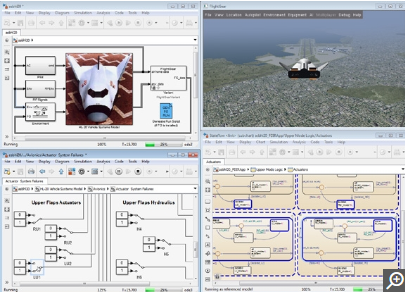
\includegraphics[scale=1]{simulinkModel.png}
    			\caption{Mô hình phương tiện hàng không vũ trụ và logic điều khiển quản lý lỗi bằng Simulink}
    \end{figure}
    Mô hình hóa và mô phỏng hành vi hệ thống động với Matlab, Simulink và Simscape
    Mô hình hóa là một cách để tạo ra một đại diện ảo của một hệ thống trong thế giới thực bao gồm phần mềm và phần cứng. Nếu các thành phần phần mềm của mô hình này được điều khiển bởi các mối quan hệ toán học, ta có thể mô phỏng biểu diễn ảo này trong một loạt các điều kiện để xem cách nó hoạt động.
    
    
    
    Với Simulink, ta có thể dễ dàng tạo ra các mô hình khác nhau chỉ đơn giản bằng cách sử dụng sơ đồ khối với rất nhiều các khối lệnh đã được xây dựng sẵn có trong thư viện. Các biểu diễn phổ biến cho các mô hình hệ thống bao gồm sơ đồ khối, sơ đồ và biểu đồ trạng thái. Sử dụng các biểu diễn này, ta có thể mô hình hóa các hệ thống cơ điện tử, phần mềm điều khiển , thuật toán xử lý tín hiệu và hệ thống truyền thông một cách dễ dàng và trực quan, thuận tiện.
    
    	
    \subsection{Deep Learning}
    
    Với Matlab, ta có thể bắt đầu với một bộ đầy đủ các thuật toán và mô hình dựng sẵn, sau đó tạo và sửa đổi các mô hình học sâu bằng ứng dụng Deep Network Designer. Kết hợp các mô hình học tập sâu cho các vấn đề cụ thể theo miền mà không phải tạo kiến trúc mạng phức tạp từ đầu. Chỉ với một vài dòng mã Matlab , ta đã có thể áp dụng các kỹ thuật học sâu được xây dựng sẵn vào công việc của mình cho dù là thiết kế thuật toán, chuẩn bị và dán nhãn dữ liệu hay tạo mã và triển khai cho các hệ thống nhúng.
    \begin{center}
    \begin{figure}[h]
    	\centering
    		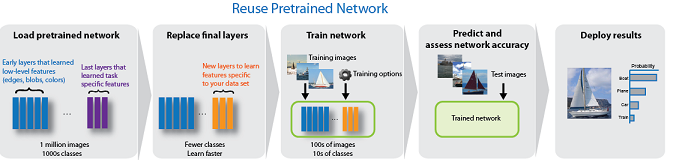
\includegraphics[scale=0.8]{deepLearning.png}
    		\caption{Sử dụng mô hình học sâu dựng sắn}
    \end{figure}
    $ \bigstar $ Ưu điểm:
    \end{center}
    \begin{itemize}
    	\item Xử lý trước dữ liệu và tự động ghi nhãn thực tế của hình ảnh, video và dữ liệu âm thanh bằng các ứng dụng.
    	\item Tăng tốc thuật toán trên  các tài nguyên  GPU, đám mây và trung tâm dữ liệu của NVIDIA mà không cần lập trình chuyên biệt.
    	\item Phối hợp với các đồng nghiệp bằng cách sử dụng các khung như TensorFlow, PyTorch và MxNet.
    	\item Mô phỏng và huấn luyện hành vi hệ thống năng động với học tăng cường.
    	\item Tạo dữ liệu thử nghiệm và đào tạo dựa trên mô phỏng từ  các mô hình Matlab và Simulink của các hệ thống vật lý.
    	
    
    
    \end{itemize}
    
    \subsection{Graphics}
    \begin{figure}[h]
    	\centering
    		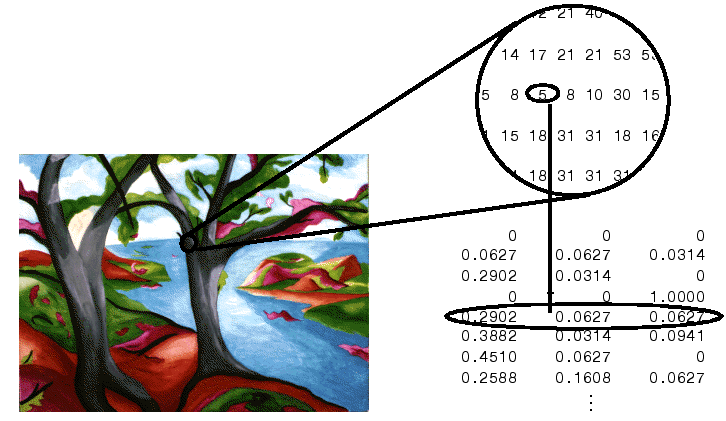
\includegraphics[scale=0.6]{resources/imageMatrix.PNG}
    		\caption{Minh họa cấu trúc của một hình ảnh được lập chỉ mục}
    \end{figure}
    	   
    Trong không gian làm việc MATLAB, hầu hết các hình ảnh được biểu diễn dưới dạng mảng hai chiều (ma trận), trong đó mỗi phần tử của ma trận tương ứng với một pixel trong hình ảnh được hiển thị. Ví dụ: một hình ảnh bao gồm 200 hàng và 300 cột của các chấm màu khác nhau được lưu trữ dưới dạng ma trận 200 x 300. Một số hình ảnh, chẳng hạn như RGB, yêu cầu mảng ba chiều, trong đó mặt phẳng thứ nhất ở chiều thứ ba đại diện cho cường độ pixel màu đỏ, mặt phẳng thứ hai biểu thị cường độ pixel màu xanh lá cây và mặt phẳng thứ ba đại diện cho cường độ pixel màu xanh. Quy ước này làm việc với các hình ảnh định dạng tệp đồ họa tương tự như làm việc với bất kỳ loại dữ liệu ma trận nào khác. Ví dụ: ta có thể chọn một pixel từ một ma trận hình ảnh bằng cách sử dụng tính năng đăng ký ma trận thông thường.
    
     Matlab cho phép tùy chỉnh đồ họa bằng cách đặt thuộc tính của các đối tượng cơ bản:
    các đối tượng đồ họa là các thành phần được Matlab sử dụng để tạo trực quan hóa dữ liệu. Mỗi đối tượng đóng một vai trò cụ thể trong màn hình đồ họa. Ví dụ, một biểu đồ đường bao gồm một đối tượng hình, một đối tượng trục và một đối tượng đường biểu đồ .Ta có thể tùy chỉnh các đối tượng đồ họa bằng cách đặt thuộc tính của chúng. Các đối tượng đồ họa được tổ chức thành một hệ thống phân cấp, như thể hiện trong sơ đồ sau. Bản chất phân cấp của các đối tượng đồ họa phản ánh sự ngăn chặn của các đối tượng bởi các đối tượng khác.
    	
    Vẽ đồ thị là một tính năng được trau chuốt trong MatLab với rất nhiều kiểu đồ thị khác nhau như biểu đồ dạng đường, biểu đồ chấm điểm, các lớp màu (patch) hai chiều, đường đồng mức và các đường cong, mặt cong ba chiều. Ngoài ra MatLab còn cung cấp giao diện để người dùng trực tiếp biên tập hình vẽ, điền vào các ghi chú theo ý muốn, các tùy chỉnh theo ý muốn. 
    	
    Matlab cho phép ta vẽ đồ thị từ các mảng dữ liệu hay vẽ các mặt từ một ma trận bằng các lệnh khác nhau, tạo ra các kiểu đồ thị khác nhau theo ý muốn của chúng ta. Matlab có các hàm đồ họa để vẽ nên các đặc tuyến bất kì trê mặt phẳng 2D hoặc 3D, cho phép tạo ra đối tượng đồ họa có thể điều khiển được. Matlab có thể được dùng để biểu diễn độ sâu của địa hình hau một trường trong không gian nói chung (như nhiệt độ, khí áp, ...).
    
   \begin{figure}[h]
    	\centering
    		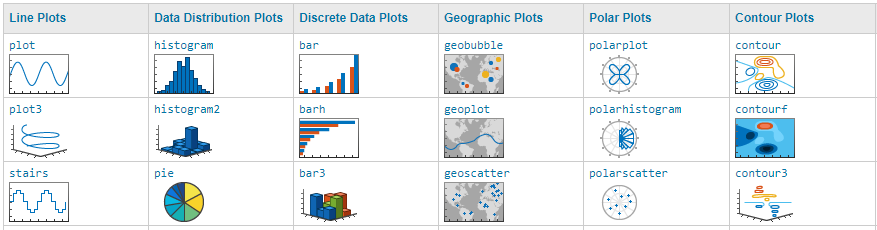
\includegraphics[scale=0.6]{graphType.png}
    		\caption{Vô vàn các loại đồ thị khác nhau}
    \end{figure}
 
    \section{\LaTeX}
    
    \LaTeX\  là một hệ thống soạn thảo bao gồm các tính năng được thiết kế để sản xuất tài liệu khoa học và kĩ thuật. \LaTeX\  là tiêu chuẩn, được sử dụng rộng rãi cho việc truyền thông và xuất bản các tài liệu khoa học trong nhiều lĩnh vực.
    \LaTeX\  rất phù hợp cho việc tạo ra các bài báo, báo cáo, luận văn, sách, hoặc các bài trình diễn, đặc biệt các tài liệu có nhiều các công thức toán học. \LaTeX\  còn cho phép chèn các hình ảnh, bảng biểu, công thức toán học vào văn bản chữ mà vẫn giữ được định dạng trang. Các tài liệu soạn thảo bằng \LaTeX\  có chất lượng định dạng cao, trông đẹp mắt và chất lượng bản in rất tốt.
    LaTeX khác với các hệ thống sắp chữ khác ở chỗ ta chỉ cần nói với nó cấu trúc logic và ngữ nghĩa của văn bản. Sau đó, nó xuất phát từ hình thức đánh máy của văn bản theo các quy tắc được đưa ra trong tệp lớp tài liệu và trong các tệp kiểu khác nhau. \LaTeX\  cho phép người dùng tạo cấu trúc tài liệu với nhiều cấu trúc phân cấp khác nhau, bao gồm các chương, phần, phần phụ và đoạn văn, như bản báo cáo này được chia làm 4 chương chính được ghi rõ ở phần mục lục. 
    Với \LaTeX, ta cung cấp các lớp văn bản khác nhau như article, thuyết trình với beamer class, viết sách với book class, ... tạo điều kiện trình bày tài liệu một cách chuyên nghiệp và thuận tiện. Ta còn có thể thêm đồ họa bằng cách sử dụng các gói lệnh như TikZ. TikZ là một trong các gói lệnh (packages) vẽ hình phổ biến và được yêu thích nhất trong LaTeX và có thể cho bạn vẽ bất cứ thứ gì mình thích vào \LaTeX . Nó được sử dụng rộng rãi trong các bài báo, văn bản và các bài trình chiếu bằng \LaTeX\ 
    \begin{center}
    $ \bigstar $ Ưu điểm:
    \end{center}
    \begin{itemize}
    	\item Các mô hình trình bày bản in chuyên nghiệp có sẵn giúp tài liệu trông chuyên nghiệp.
    	\item  Việc soạn thảo các công thức toán học, kỹ thuật được hỗ trợ đến tối đa.
    	\item Người sử dụng chỉ cần học một số lệnh dễ nhớ để xác định cấu trúc logic của tài liệu. Người dùng không phải suy nghĩ nhiều đến việc trình bày bản in vì việc này được làm một cách tự động.
    	\item Các cấu trúc phức tạp như chú thích, tham chiếu, biểu bảng, mục lục, ... được tạo ra dễ dàng.
    	\item Có thể sử dụng nhiều gói add-on package miễn phí nhằm bổ sung những tính năng mà \LaTeX\  không hỗ trợ trực tiếp.
    \end{itemize}
    
    \begin{center}
    $ \bigstar $ Nhược điểm:
    \end{center}
    \begin{itemize}
    	\item Không nhìn thấy văn bản hiển thị khi đang gõ.
    	\item Phải ghi nhớ các tên lệnh.
    	\item Mất nhiều thời gian hơn so với các chương trình soạn thảo văn bản thông thường.
    \end{itemize}
    



    

    %===================================================================================
    \chapter{Những thuận lợi, thách thức và yêu cầu của sinh viên Toán - Tin trong thời kì Cách mạng công nghiệp 4.0}
    
        Hiện nay, thế giới và Việt Nam đang chứng kiến những sự thay đổi vượt bậc trong thời đại công nghệ số của cuộc cách mạng công nghiệp lần thứ tư (CMCN 4.0) và tầm ảnh hưởng sâu rộng của khoa học công nghệ đến đời sống con người. Bản chất của CMCN 4.0 chính là sự ứng dụng công nghệ, khoa học dữ liệu và sử dụng trí tuệ nhân tạo phục vụ đời sống xã hội - cũng chính là một trong những nhánh của Toán học ứng dụng, do đó, sinh viên Toán Tin đang có một lợi thế rất lớn, bởi sinh viên sẽ được trang bị một nền tảng và các công cụ toán sẵn có, song song với các hệ thống máy tính ngày càng hiện đại. Họ cũng là những người đóng vai trò chủ chốt trong lĩnh vực R$\&$D (Nghiên cứu và phát triển) các thuật toán mới ưu việt và hiệu quả hơn. Bên canh những thuận lợi kể trên, cuộc CMCN 4.0 cũng đem lại không ít thách thức và khó khăn. Chẳng hạn:
        
        \begin{itemize}
            \item Tốc độ lỗi thời của công nghệ ngày càng nhanh, trước kia một công nghệ có thể kéo dài 15-20 năm hoặc hơn, bây giờ đã rút ngắn lại chỉ còn vài năm, thậm chí chưa đến 1 năm.
            \item Sự tinh xảo, hoàn thiện và tính chuyên biệt hóa của công nghệ ngày càng cao, yêu cầu sự phối kết hợp của không chỉ một, hai mà là nhiều ngành nghề khác nhau.
        \end{itemize}
    
        Đứng trước những thuận lợi và thách thức trên, ngoài việc nắm chắc các kiến thức chuyên môn, nền tảng, sinh viên Toán - Tin cần có những phẩm chất và kỹ năng sau đây:
        
        \begin{itemize}
            \item Khả năng ứng dụng khoa học công nghệ vào thực tiễn
            \item Kỹ năng làm việc thực tế, chủ động và sáng tạo trong công việc
            \item Khả năng ngoại ngữ, đặc biệt là tiếng Anh.
            \item Các kỹ năng tương lai, bao gồm 10 kỹ năng sau đây
            \begin{itemize}
                \item Kỹ năng giải quyết vấn đề - \textit{Problem - solving skill}
                \item Kỹ năng tư duy phản biện - \textit{Critical thinking skill}
                \item Kỹ năng sáng tạo - \textit{Creative skill}
                \item Kỹ năng quản lý nhân lực - \textit{Human resource management skill}
                \item Kỹ năng làm việc nhóm - \textit{Teamwork}
                \item Tư duy cảm xúc - \textit{Emotional Intelligence}
                \item Kỹ năng đánh giá $\&$ đưa ra quyết định - \textit{Review $\&$ Decision-making skill}
                \item Kỹ năng tư duy dịch vụ - \textit{Service thinking skill}
                \item Kỹ năng thương lượng - \textit{Negotiation Skill}
                \item Khả năng nhận thức linh hoạt - \textit{Cognitive Flexibility skill}
            \end{itemize}
            
            
        \end{itemize}
        
        
    \textbf{{\large}}\\[3cm]
    \begin{center}
        \Huge \texttt{ \textbf{Thank you and Good bye} }
    \end{center}
    
    \newpage
    \addcontentsline{toc}{chapter}{Taì liệu tham khảo}
    \begin{center}
        \huge \textbf{TÀI LIỆU THAM KHẢO}
    \end{center}
    \begin{itemize}
        \item Slide bài giảng của thầy \textit{Phạm Hồng Thanh}, Phó giám đốc Học viện Viettel
        \item Slide bài giảng của cô \textit{Nghiêm Thị Lan Phương}, K44/SAMI/HUST - \textit{CM4.0 và động lực}
        \item Slide bài giảng của thầy \textit{Bùi Kiên Cường}, KSTN/SAMI/HUST, Phó giám đốc VinID
        \item Chương trình đào tạo Cử nhân HT Toán Tin, thầy \textit{Nguyễn Cảnh Nam, Đỗ Đức Thuận}, SAMI/HUST 
        \item Chương trình 1439 - CTTN-Toán tin-2019, 
        
        \url{https://ctt-sis.hust.edu.vn/Students/StudentProgram.aspx} \textit{(yêu cầu đăng nhập)}
        
        \item Giới thiệu chung về Matlab,
        
        \url{https://www.mathworks.com/}
       
        \item Học sâu trong Matlab,
        
        \url{https://www.mathworks.com/help/deeplearning/ug/deep-learning-in-matlab.html}
        \item Mô hình hóa và mô phỏng trong Matlab,
        
        \url{https://www.mathworks.com/discovery/modeling-and-simulation.html}
        \item Đồ họa trong Matlab,
        
        \url{https://www.mathworks.com/help/matlab/graphics.html}
        \item Giới thiệu tổng quan về \LaTeX ,
        
        \url{https://viblo.asia/p/tong-quan-ve-latex-n7prv3N8GKod}
        
        \url{https://www.latex-project.org/}
        
        \item Tầm quan trọng của Toán Tin
        
        \url{https://www.wikipedia.org/}
        
        \url{http://sami.hust.edu.vn}
        \item Ứng dụng của Toán Tin
        
        \url{http://viethanit.edu.vn}
        
        \url{https://timviecit.net}
        
    \end{itemize}
    

\end{document}
